\documentclass[12pt]{article}
\usepackage{tikz}
\usetikzlibrary{shadings,patterns}

\author{Binit Pandit}
\title{Drawing in \LaTeX\ using PGF/TikZ}
\date{}

\begin{document}
\maketitle\vskip-25pt\hrule\vskip10pt

%\begin{tikzpicture}[options]
%\path[optional1][optional1] <specifications> ;
%\end{tikzpicture}

\begin{tikzpicture}
    \draw (0,0) rectangle (3,4);
\end{tikzpicture}
\vskip25pt

\begin{tikzpicture}
    \fill[color=yellow] (0,0) rectangle (3,4);
\end{tikzpicture}
\vskip25pt

\begin{tikzpicture}
    \fill[color=yellow] (0,0) rectangle (3,4);
    \draw[color=red] (0,0) rectangle (3,4);
\end{tikzpicture}
\vskip25pt
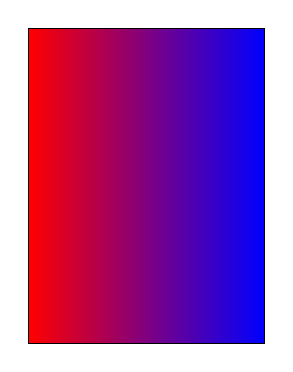
\begin{tikzpicture}
    %\shade[shading=ball] (0,0) rectangle (3,4);
    \shade[left color = red, right color = blue] (0,0) rectangle (3,4);
    \draw (0,0) rectangle (3,4);
\end{tikzpicture}
\vskip25pt
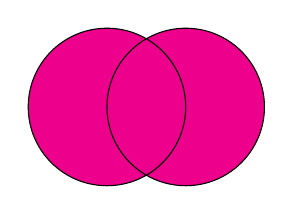
\begin{tikzpicture}
    \fill [color=magenta] (0,0) circle[radius=1cm] (1,0) circle[radius=1cm];
    \draw (0,0) circle[radius=1cm] (1,0) circle[radius=1cm];
\end{tikzpicture}
\vskip25pt
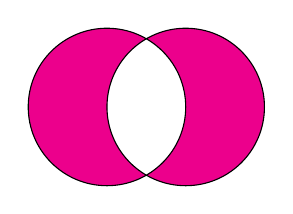
\begin{tikzpicture}
    \fill [color=magenta, even odd rule] (0,0) circle[radius=1cm] (1,0) circle[radius=1cm];
    \draw (0,0) circle[radius=1cm] (1,0) circle[radius=1cm];
\end{tikzpicture}
\vskip25pt
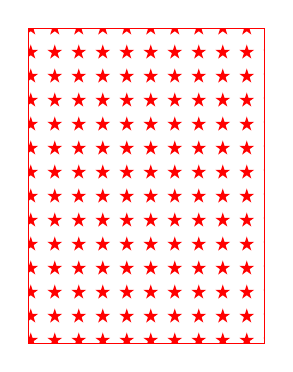
\begin{tikzpicture}
    %\pattern [pattern=dots] (0,0) rectangle (3,4);
    \pattern [pattern=fivepointed stars,pattern color = red] (0,0) rectangle (3,4);
    \draw [color=red] (0,0) rectangle (3,4);
\end{tikzpicture}
\end{document}